\section{Transformation der Eingabevariablen}

\subsection{Vorgehen}
Gemäß der Aufgabenstellung in der Template-Datei, experimentierten wir mit den
Transformationen "`Decorrelate"' (D), "`Gauß"' (G), und "`Normalise"' (N).
Um heraus zu finden, ob sie einen Einfluss auf das Ergebnis haben, wendeten wir
sie in allen Kombinationen und Reihenfolgen auf den Input an und evaluierten den AMS-Wert.

\subsection{Auswertung}
Die Ergebnisse sind in Abbildung \ref{fig:ams_over_transforamtion} gezeigt. Man
sieht, dass es für die Fischer-Methode Sinn macht, die Daten zu dekorrelieren
und zu Normalisieren. Die Reihenfolge hat keine Auswirkungen. Bei der
BDT-Methode verschlechtern die Transformationen das Ergebnis. Außerdem gab es
bei dieser Methode bei manchen Transformationen einen Programmfehler, den wir
nicht weiter untersucht haben. In Abbildung \ref{fig:ams_over_transforamtion}
sind nur die erfolgreichen Abläufe der BDT-Methode gelistet und deshalb weniger
als bei der Fischer-Methode.





%\usepackage{graphics} is needed for \includegraphics
\begin{figure}[htp]
\begin{center}
  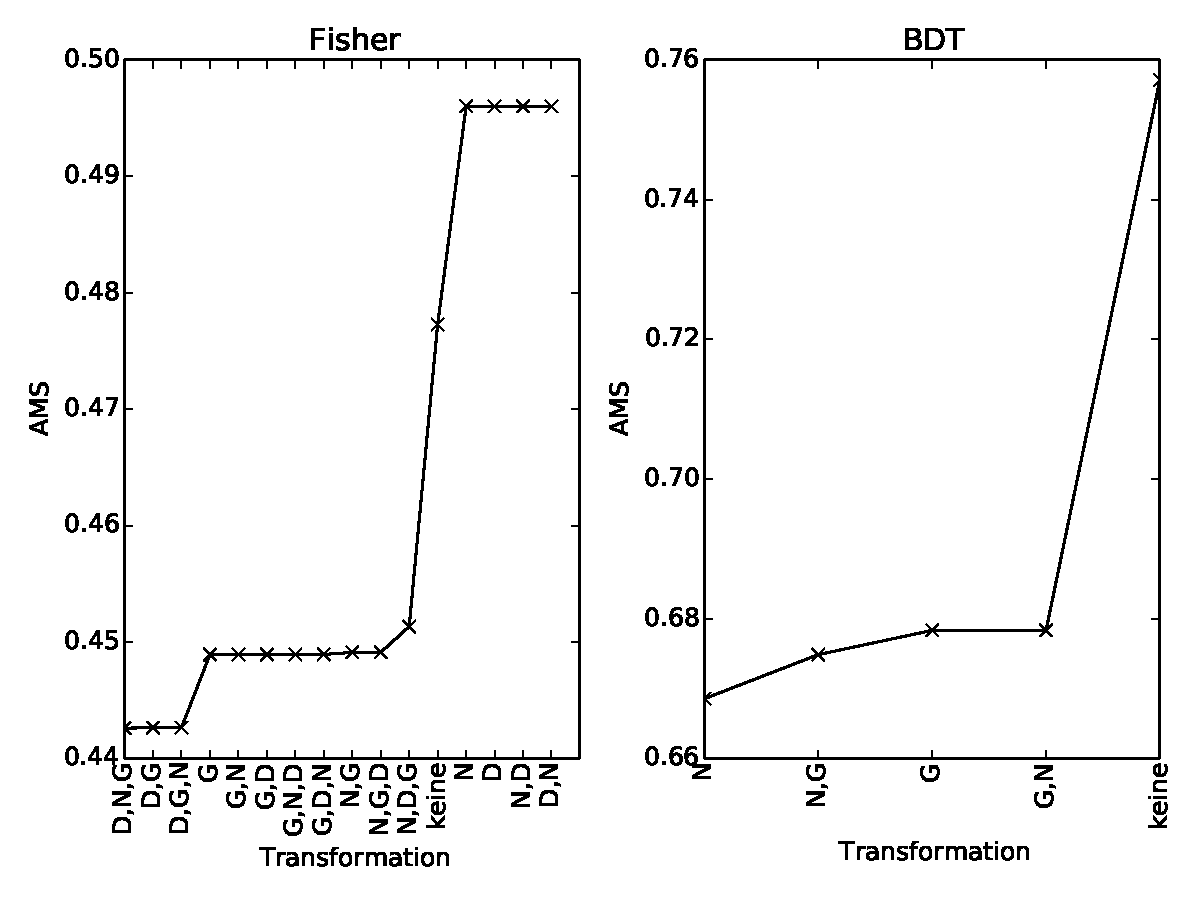
\includegraphics[width=\linewidth]{sections/input_transformations/var_transform_ranking.pdf}
  \caption[AMS über Transformation der Eingabevariablen]{AMS über Transformation der Eingabevariablen.}
  \label{fig:ams_over_transforamtion}
\end{center}
\end{figure}

